% Options for packages loaded elsewhere
\PassOptionsToPackage{unicode}{hyperref}
\PassOptionsToPackage{hyphens}{url}
\PassOptionsToPackage{dvipsnames,svgnames,x11names}{xcolor}
%
\documentclass[
  beamerpaper,
  DIV=11,
  numbers=noendperiod,
  aspectratio=54]{scrreprt}

\usepackage{amsmath,amssymb}
\usepackage{iftex}
\ifPDFTeX
  \usepackage[T1]{fontenc}
  \usepackage[utf8]{inputenc}
  \usepackage{textcomp} % provide euro and other symbols
\else % if luatex or xetex
  \usepackage{unicode-math}
  \defaultfontfeatures{Scale=MatchLowercase}
  \defaultfontfeatures[\rmfamily]{Ligatures=TeX,Scale=1}
\fi
\usepackage{lmodern}
\ifPDFTeX\else  
    % xetex/luatex font selection
  \setmonofont[Scale=0.6]{Source Code Pro}
\fi
% Use upquote if available, for straight quotes in verbatim environments
\IfFileExists{upquote.sty}{\usepackage{upquote}}{}
\IfFileExists{microtype.sty}{% use microtype if available
  \usepackage[]{microtype}
  \UseMicrotypeSet[protrusion]{basicmath} % disable protrusion for tt fonts
}{}
\makeatletter
\@ifundefined{KOMAClassName}{% if non-KOMA class
  \IfFileExists{parskip.sty}{%
    \usepackage{parskip}
  }{% else
    \setlength{\parindent}{0pt}
    \setlength{\parskip}{6pt plus 2pt minus 1pt}}
}{% if KOMA class
  \KOMAoptions{parskip=half}}
\makeatother
\usepackage{xcolor}
\setlength{\emergencystretch}{3em} % prevent overfull lines
\setcounter{secnumdepth}{-\maxdimen} % remove section numbering
% Make \paragraph and \subparagraph free-standing
\ifx\paragraph\undefined\else
  \let\oldparagraph\paragraph
  \renewcommand{\paragraph}[1]{\oldparagraph{#1}\mbox{}}
\fi
\ifx\subparagraph\undefined\else
  \let\oldsubparagraph\subparagraph
  \renewcommand{\subparagraph}[1]{\oldsubparagraph{#1}\mbox{}}
\fi


\providecommand{\tightlist}{%
  \setlength{\itemsep}{0pt}\setlength{\parskip}{0pt}}\usepackage{longtable,booktabs,array}
\usepackage{calc} % for calculating minipage widths
% Correct order of tables after \paragraph or \subparagraph
\usepackage{etoolbox}
\makeatletter
\patchcmd\longtable{\par}{\if@noskipsec\mbox{}\fi\par}{}{}
\makeatother
% Allow footnotes in longtable head/foot
\IfFileExists{footnotehyper.sty}{\usepackage{footnotehyper}}{\usepackage{footnote}}
\makesavenoteenv{longtable}
\usepackage{graphicx}
\makeatletter
\def\maxwidth{\ifdim\Gin@nat@width>\linewidth\linewidth\else\Gin@nat@width\fi}
\def\maxheight{\ifdim\Gin@nat@height>\textheight\textheight\else\Gin@nat@height\fi}
\makeatother
% Scale images if necessary, so that they will not overflow the page
% margins by default, and it is still possible to overwrite the defaults
% using explicit options in \includegraphics[width, height, ...]{}
\setkeys{Gin}{width=\maxwidth,height=\maxheight,keepaspectratio}
% Set default figure placement to htbp
\makeatletter
\def\fps@figure{htbp}
\makeatother

\usepackage{titling}
\usepackage{fancyhdr, blindtext}
\usepackage{xcolor}
\usepackage{soul}
\usepackage{pagecolor}
\usepackage{booktabs}
\usepackage{longtable}
\usepackage{array}
\usepackage{multirow}
\usepackage{wrapfig}
\usepackage{float}
\usepackage{colortbl}
\usepackage{pdflscape}
\usepackage{tabu}
\usepackage{threeparttable}
\usepackage{threeparttablex}
\usepackage[normalem]{ulem}
\usepackage{makecell}
\usepackage{tcolorbox}
\usepackage[]{Oswald}
\usepackage{lipsum}

\definecolor{merkgreen}{RGB}{202,211,68}
\definecolor{merkdarkgreen}{RGB}{52,93,70}
\definecolor{merkyellow}{RGB}{247,233,9}

\definecolor{bggray}{rgb}{0.95,0.95,0.95}
\pagestyle{fancy}
\pretitle{\begin{center}
  
\includegraphics[width=5in,height=3.5in]{../img/logo_Merkanzia.pdf}\LARGE\\}
  \pagecolor{merkdarkgreen}
\posttitle{\end{center}}
\fancyhf{}
\newpage
\newpagecolor{merkgreen}
% \begin{tcolorbox}[
%     title="Prezzi",
% %   opacityback=1,  % this does not work
% %   colback=white,  % this is not what I want
% ]
\fancyfoot[R]{\footnotesize \textit{www.merkanzia.com info@merkanzia.com}}
\fancyfoot[L]{\footnotesize \textit{Merkanzia GmbH, La Toscana in Svizzera}}
\usepackage{booktabs}
\usepackage{longtable}
\usepackage{array}
\usepackage{multirow}
\usepackage{wrapfig}
\usepackage{float}
\usepackage{colortbl}
\usepackage{pdflscape}
\usepackage{tabu}
\usepackage{threeparttable}
\usepackage{threeparttablex}
\usepackage[normalem]{ulem}
\usepackage{makecell}
\usepackage{xcolor}
\KOMAoption{captions}{tableheading}
\makeatletter
\makeatother
\makeatletter
\makeatother
\makeatletter
\@ifpackageloaded{caption}{}{\usepackage{caption}}
\AtBeginDocument{%
\ifdefined\contentsname
  \renewcommand*\contentsname{Table of contents}
\else
  \newcommand\contentsname{Table of contents}
\fi
\ifdefined\listfigurename
  \renewcommand*\listfigurename{List of Figures}
\else
  \newcommand\listfigurename{List of Figures}
\fi
\ifdefined\listtablename
  \renewcommand*\listtablename{List of Tables}
\else
  \newcommand\listtablename{List of Tables}
\fi
\ifdefined\figurename
  \renewcommand*\figurename{Figure}
\else
  \newcommand\figurename{Figure}
\fi
\ifdefined\tablename
  \renewcommand*\tablename{Table}
\else
  \newcommand\tablename{Table}
\fi
}
\@ifpackageloaded{float}{}{\usepackage{float}}
\floatstyle{ruled}
\@ifundefined{c@chapter}{\newfloat{codelisting}{h}{lop}}{\newfloat{codelisting}{h}{lop}[chapter]}
\floatname{codelisting}{Listing}
\newcommand*\listoflistings{\listof{codelisting}{List of Listings}}
\makeatother
\makeatletter
\@ifpackageloaded{caption}{}{\usepackage{caption}}
\@ifpackageloaded{subcaption}{}{\usepackage{subcaption}}
\makeatother
\makeatletter
\@ifpackageloaded{tcolorbox}{}{\usepackage[skins,breakable]{tcolorbox}}
\makeatother
\makeatletter
\@ifundefined{shadecolor}{\definecolor{shadecolor}{rgb}{.97, .97, .97}}
\makeatother
\makeatletter
\makeatother
\makeatletter
\makeatother
\ifLuaTeX
  \usepackage{selnolig}  % disable illegal ligatures
\fi
\IfFileExists{bookmark.sty}{\usepackage{bookmark}}{\usepackage{hyperref}}
\IfFileExists{xurl.sty}{\usepackage{xurl}}{} % add URL line breaks if available
\urlstyle{same} % disable monospaced font for URLs
\hypersetup{
  pdftitle={Catalogo Prezzi B2B},
  colorlinks=true,
  linkcolor={blue},
  filecolor={Maroon},
  citecolor={Blue},
  urlcolor={Blue},
  pdfcreator={LaTeX via pandoc}}

\title{Catalogo Prezzi B2B}
\usepackage{etoolbox}
\makeatletter
\providecommand{\subtitle}[1]{% add subtitle to \maketitle
  \apptocmd{\@title}{\par {\large #1 \par}}{}{}
}
\makeatother
\subtitle{Merkanzia GmbH - La Toscana in Svizzera}
\author{}
\date{August 7, 2023\\
\strut \\
\strut \\
info@merkanzia.com}

\begin{document}
\maketitle
\ifdefined\Shaded\renewenvironment{Shaded}{\begin{tcolorbox}[sharp corners, boxrule=0pt, frame hidden, enhanced, interior hidden, borderline west={3pt}{0pt}{shadecolor}, breakable]}{\end{tcolorbox}}\fi

\renewcommand{\arraystretch}{1.6}

\begin{table}

\caption{\label{tbl-panel-cla-aro}Caseificio La Fonte (Asciano -
Siena)}\begin{minipage}[t]{0.60\linewidth}
\subcaption{\label{tbl-panel-cla-aro-1}I Classici }

\tabularnewline

\fontsize{9.5}{11.5}\selectfont
\begin{tabular}{>{\raggedright\arraybackslash}p{3.25cm}>{\raggedright\arraybackslash}p{2.25cm}l}
\toprule
\textbf{Prodotto} & \textbf{Quantità} & \textbf{CHF/Kg}\\
\midrule
\textbf{\em{I Classici di La Fonte}} & \textbf{Una forma 1,5 kg} & \textbf{}\\
\cmidrule{1-3}
 & < 10 kg & 32.05\\

\multirow[t]{-2}{3.25cm}{\raggedright\arraybackslash \em{Sua Eccellenza il Fresco (20gg)}} & > 10kg & 28.84\\
\cmidrule{1-3}
 & < 10 kg & 35\\

\multirow[t]{-2}{3.25cm}{\raggedright\arraybackslash \em{Sua Eccellenza il Semi Stagionato (60gg)}} & > 10kg & 31.5\\
\cmidrule{1-3}
 & < 10 kg & 37.33\\

\multirow[t]{-2}{3.25cm}{\raggedright\arraybackslash \em{Sua Eccellenza lo Stagionato (90gg)}} & > 10kg & 33.6\\
\bottomrule
\multicolumn{3}{l}{\rule{0pt}{1em}\textit{Note: }}\\
\multicolumn{3}{l}{\rule{0pt}{1em}gg: Giorni Stagionatura}\\
\multicolumn{3}{l}{\rule{0pt}{1em}}\\
\end{tabular}

\end{minipage}%
%
\begin{minipage}[t]{0.40\linewidth}

\raisebox{-\height}{

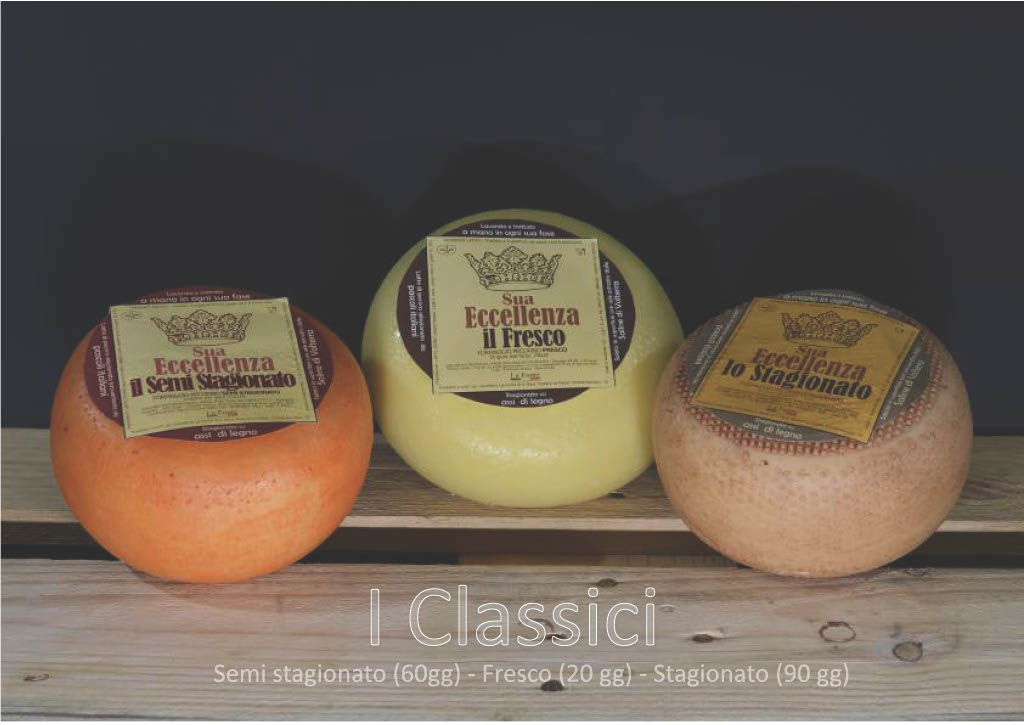
\includegraphics{../img/LaFonte_IClassici1024_1.jpeg}

}

\end{minipage}%
\newline
\begin{minipage}[t]{0.60\linewidth}
\subcaption{\label{tbl-panel-cla-aro-2}Gli Aromatizzati }

\tabularnewline

\fontsize{9.5}{11.5}\selectfont
\begin{tabular}{>{\raggedright\arraybackslash}p{3.25cm}>{\raggedright\arraybackslash}p{2.25cm}l}
\toprule
\textbf{Prodotto} & \textbf{Quantità} & \textbf{CHF/Kg}\\
\midrule
\textbf{\em{Gli Aromatizzati di La Fonte}} & \textbf{Una forma 1,5-3 kg} & \textbf{}\\
\cmidrule{1-3}
 & < 10 kg & 38.03\\

\multirow[t]{-2}{3.25cm}{\raggedright\arraybackslash \em{Sua Eccellenza Il Pepe Nero (100gg)}} & > 10kg & 34.23\\
\cmidrule{1-3}
 & < 10 kg & 38.03\\

\multirow[t]{-2}{3.25cm}{\raggedright\arraybackslash \em{Sua Eccellenza Il Pistacchio (20gg)}} & > 10kg & 34.23\\
\cmidrule{1-3}
 & < 10 kg & 47.07\\

\multirow[t]{-2}{3.25cm}{\raggedright\arraybackslash \em{Sua Eccellenza Il Tartufo (20gg)}} & > 10kg & 42.37\\
\cmidrule{1-3}
 & < 10 kg & 35.93\\

\multirow[t]{-2}{3.25cm}{\raggedright\arraybackslash \em{Sua Eccellenza Il Piccante (20gg)}} & > 10kg & 32.34\\
\cmidrule{1-3}
 & < 10 kg & 38.03\\

\multirow[t]{-2}{3.25cm}{\raggedright\arraybackslash \em{Sua Eccellenza La Castagna (60gg)}} & > 10kg & 34.23\\
\bottomrule
\multicolumn{3}{l}{\rule{0pt}{1em}\textit{Note: }}\\
\multicolumn{3}{l}{\rule{0pt}{1em}gg: Giorni Stagionatura}\\
\multicolumn{3}{l}{\rule{0pt}{1em}}\\
\end{tabular}

\end{minipage}%
%
\begin{minipage}[t]{0.40\linewidth}

\raisebox{-\height}{

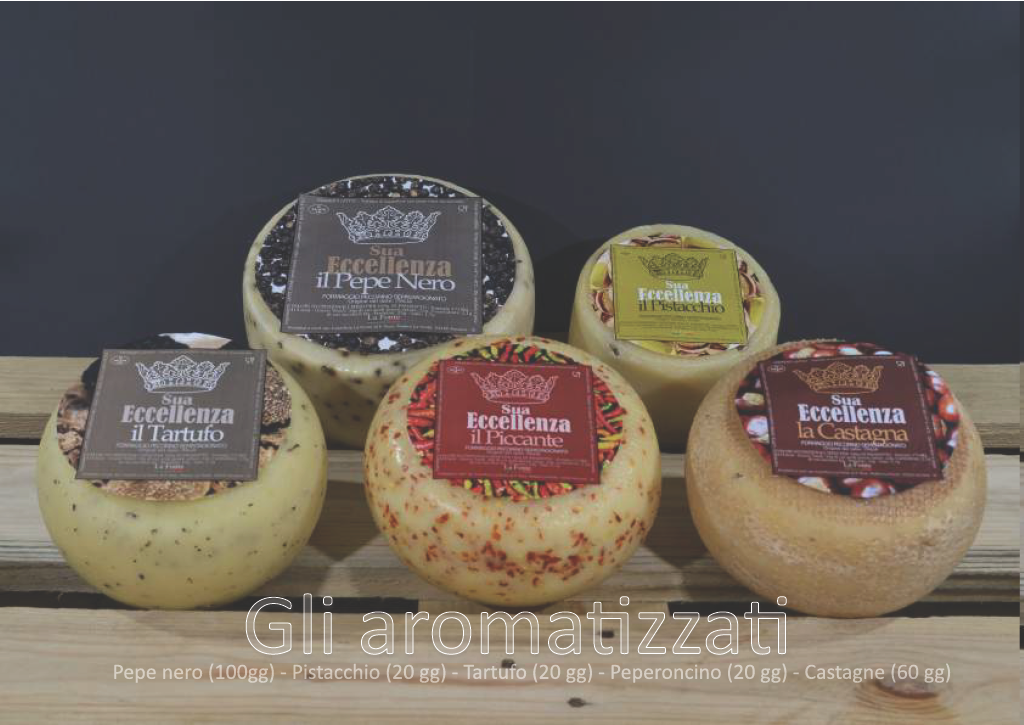
\includegraphics[width=2.44in,height=\textheight]{../img/LaFonte_gliaromatizzati1024_1.png}

}

\end{minipage}%

\end{table}

\renewcommand{\arraystretch}{1.6}

\begin{table}

\caption{\label{tbl-panel-aff-grare}Caseificio La Fonte (Asciano -
Siena)}\begin{minipage}[t]{0.60\linewidth}
\subcaption{\label{tbl-panel-aff-grare-1}Gli Affinati }

\tabularnewline

\fontsize{9.5}{11.5}\selectfont
\begin{tabular}{>{\raggedright\arraybackslash}p{3.25cm}>{\raggedright\arraybackslash}p{2.25cm}l}
\toprule
\textbf{Prodotto} & \textbf{Quantità} & \textbf{CHF/Kg}\\
\midrule
\textbf{\em{Gli Affinati di La Fonte}} & \textbf{Una forma 1,5-3 kg} & \textbf{}\\
\cmidrule{1-3}
 & < 10 kg & 38.03\\

\multirow[t]{-2}{3.25cm}{\raggedright\arraybackslash \em{Sua Eccellenza Il Foglia di Noce (90gg)}} & > 10kg & 34.23\\
\cmidrule{1-3}
 & < 10 kg & 38.49\\

\multirow[t]{-2}{3.25cm}{\raggedright\arraybackslash \em{Sua Eccellenza Il Re Fieno (70gg)}} & > 10kg & 34.64\\
\cmidrule{1-3}
 & < 10 kg & 38.03\\

\multirow[t]{-2}{3.25cm}{\raggedright\arraybackslash \em{Sua Eccellenza Il Germe di grano (60+45gg)}} & > 10kg & 34.23\\
\cmidrule{1-3}
 & < 10 kg & 38.03\\

\multirow[t]{-2}{3.25cm}{\raggedright\arraybackslash \em{Sua Eccellenza Le Vinacce (90+4gg)}} & > 10kg & 34.23\\
\cmidrule{1-3}
 & < 10 kg & 38.03\\

\multirow[t]{-2}{3.25cm}{\raggedright\arraybackslash \em{Sua Eccellenza Il Peparello (90gg)}} & > 10kg & 34.23\\
\bottomrule
\multicolumn{3}{l}{\rule{0pt}{1em}\textit{Note: }}\\
\multicolumn{3}{l}{\rule{0pt}{1em}gg: Giorni Stagionatura}\\
\multicolumn{3}{l}{\rule{0pt}{1em}}\\
\end{tabular}

\end{minipage}%
%
\begin{minipage}[t]{0.40\linewidth}

\raisebox{-\height}{

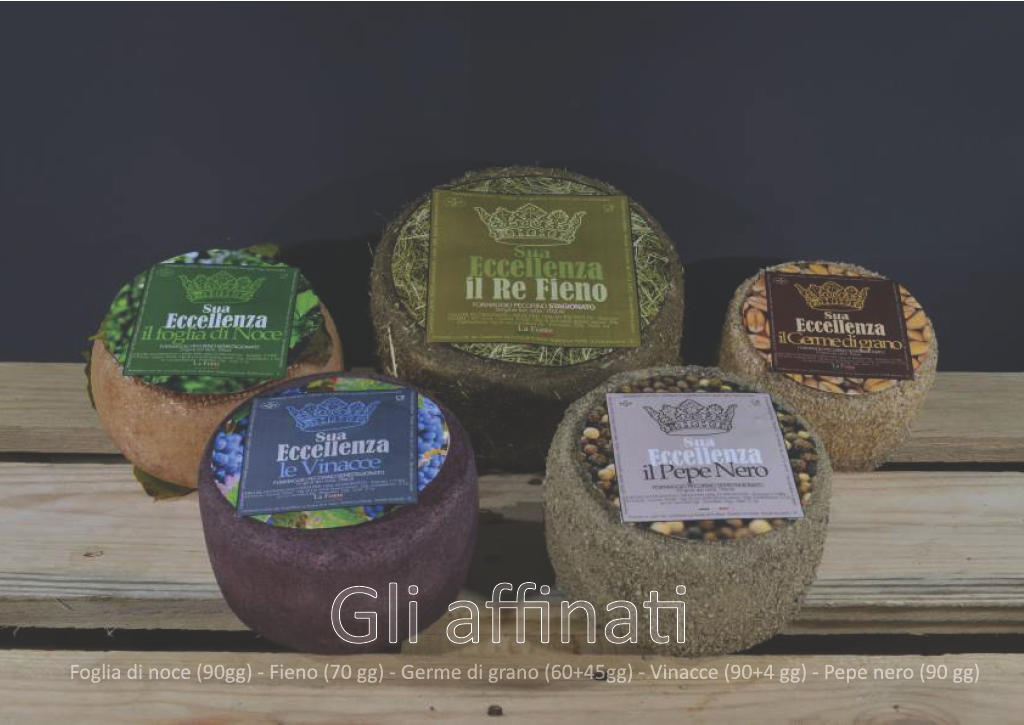
\includegraphics[width=2.44in,height=\textheight]{../img/LaFonte_GliAffinati1024_1.png}

}

\end{minipage}%
\newline
\begin{minipage}[t]{0.60\linewidth}
\subcaption{\label{tbl-panel-aff-grare-2}Il Grande ed i Re }

\tabularnewline

\fontsize{9.5}{11.5}\selectfont
\begin{tabular}{>{\raggedright\arraybackslash}p{3.25cm}>{\raggedright\arraybackslash}p{2.25cm}l}
\toprule
\textbf{Prodotto} & \textbf{Quantità} & \textbf{CHF/Kg}\\
\midrule
\textbf{\em{Il Grande e i Re}} & \textbf{Una forma 1,5-3 kg} & \textbf{}\\
\cmidrule{1-3}
 & < 10 kg & 37.79\\

\multirow[t]{-2}{3.25cm}{\raggedright\arraybackslash \em{Sua Eccellenza Il Grande (90gg)}} & > 10kg & 34.01\\
\cmidrule{1-3}
 & < 10 kg & 46.14\\

\multirow[t]{-2}{3.25cm}{\raggedright\arraybackslash \em{Sua Eccellenza Il Re Sole (200gg)}} & > 10kg & 41.53\\
\cmidrule{1-3}
 & < 10 kg & 38.71\\

\multirow[t]{-2}{3.25cm}{\raggedright\arraybackslash \em{Sua Eccellenza Il Re Grotta (90+60gg)}} & > 10kg & 34.84\\
\bottomrule
\multicolumn{3}{l}{\rule{0pt}{1em}\textit{Note: }}\\
\multicolumn{3}{l}{\rule{0pt}{1em}gg: Giorni Stagionatura}\\
\multicolumn{3}{l}{\rule{0pt}{1em}}\\
\end{tabular}

\end{minipage}%
%
\begin{minipage}[t]{0.40\linewidth}

\raisebox{-\height}{

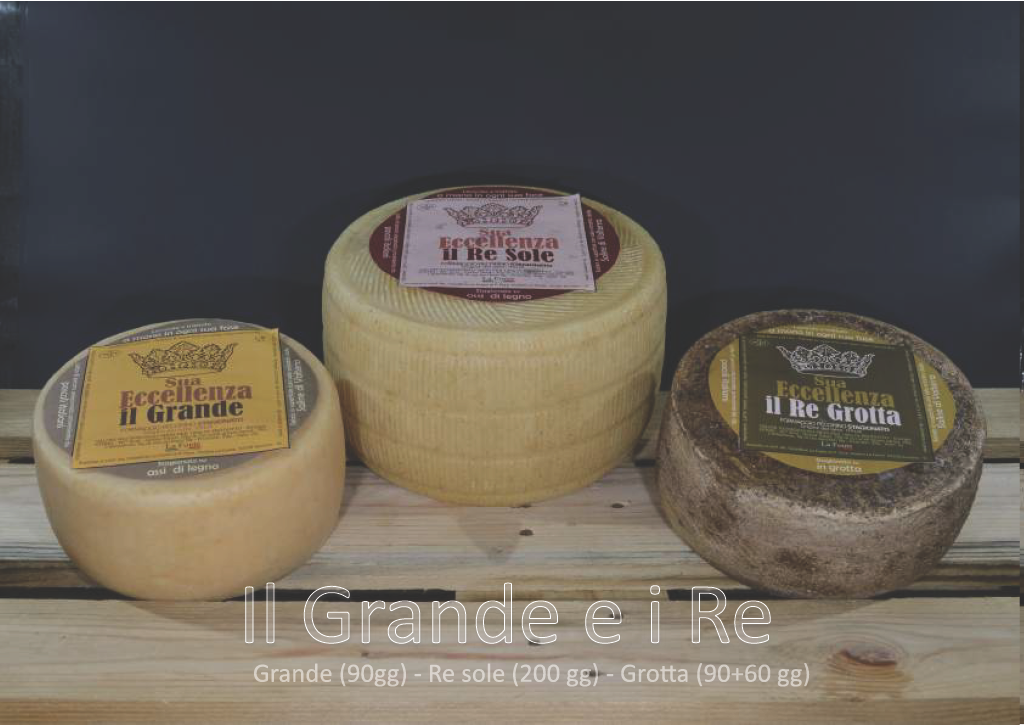
\includegraphics[width=2.44in,height=\textheight]{../img/IlGrande1024_1.png}

}

\end{minipage}%

\end{table}

\renewcommand{\arraystretch}{1.6}

\begin{table}

\caption{\label{tbl-panel-latt}Caseificio La Fonte (Asciano -
Siena)}\begin{minipage}[t]{0.60\linewidth}
\subcaption{\label{tbl-panel-latt-1}Linea Latte di Siena }

\tabularnewline

\fontsize{9.5}{11.5}\selectfont
\begin{tabular}{>{\raggedright\arraybackslash}p{3.25cm}>{\raggedright\arraybackslash}p{2.25cm}l}
\toprule
\textbf{Prodotto} & \textbf{Quantità} & \textbf{CHF/Kg}\\
\midrule
\textbf{\em{Linea Latte di Siena}} & \textbf{Una forma 1,5-5 kg} & \textbf{}\\
\cmidrule{1-3}
 & < 10 kg & 33.62\\

\multirow[t]{-2}{3.25cm}{\raggedright\arraybackslash \em{Cecco Latte Siena (20gg)}} & > 10kg & 30.26\\
\cmidrule{1-3}
 & < 10 kg & 34.63\\

\multirow[t]{-2}{3.25cm}{\raggedright\arraybackslash \em{Nobile Latte Siena (40gg)}} & > 10kg & 31.17\\
\cmidrule{1-3}
 & < 10 kg & 36.11\\

\multirow[t]{-2}{3.25cm}{\raggedright\arraybackslash \em{Mangia Latte Siena (70gg)}} & > 10kg & 32.5\\
\cmidrule{1-3}
 & < 10 kg & 37.1\\

\multirow[t]{-2}{3.25cm}{\raggedright\arraybackslash \em{Balzana Latte Siena (60gg)}} & > 10kg & 33.39\\
\cmidrule{1-3}
 & < 10 kg & 39.6\\

\multirow[t]{-2}{3.25cm}{\raggedright\arraybackslash \em{Tolomeo Latte Siena (90gg)}} & > 10kg & 35.64\\
\cmidrule{1-3}
 & < 10 kg & 40.32\\

\multirow[t]{-2}{3.25cm}{\raggedright\arraybackslash \em{Fieno Latte Siena (70gg)}} & > 10kg & 36.29\\
\bottomrule
\multicolumn{3}{l}{\rule{0pt}{1em}\textit{Note: }}\\
\multicolumn{3}{l}{\rule{0pt}{1em}gg: Giorni Stagionatura}\\
\multicolumn{3}{l}{\rule{0pt}{1em}}\\
\end{tabular}

\end{minipage}%
%
\begin{minipage}[t]{0.40\linewidth}

\raisebox{-\height}{

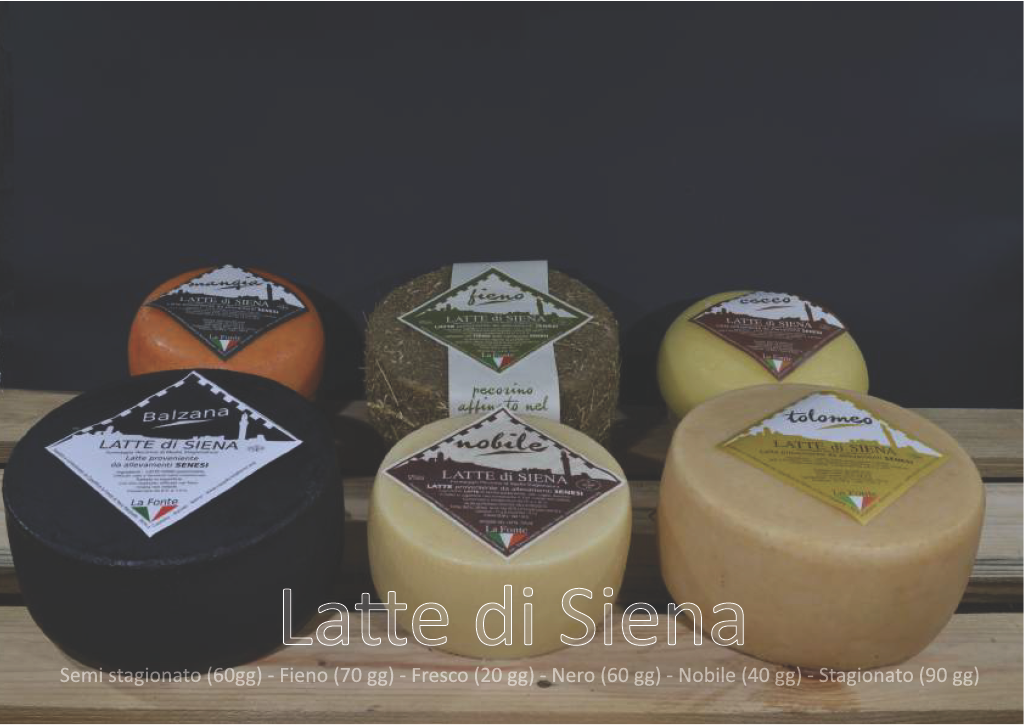
\includegraphics[width=2.44in,height=\textheight]{../img/Latte_di_siena1024_1.png}

}

\end{minipage}%

\end{table}

\begin{table}

\caption{\label{tbl-panel-mmons}Salumeria di Monte San
Savino}\begin{minipage}[t]{0.60\linewidth}
\subcaption{\label{tbl-panel-mmons-1}Porchette }

\tabularnewline

\fontsize{9.5}{11.5}\selectfont
\begin{tabular}{>{\raggedright\arraybackslash}p{3.25cm}>{\raggedright\arraybackslash}p{2.25cm}l}
\toprule
\textbf{Prodotto} & \textbf{Quantità} & \textbf{CHF/Kg}\\
\midrule
\textbf{\em{Porchetta}} & \textbf{8-11 Kg} & \textbf{}\\
\cmidrule{1-3}
 & 1/2 o 1 & 45\\

\multirow[t]{-2}{3.25cm}{\raggedright\arraybackslash \em{Tronchetto Cotto a Legna}} & >1 & 41.4\\
\bottomrule
\multicolumn{3}{l}{\rule{0pt}{1em}\textit{Note: }}\\
\multicolumn{3}{l}{\rule{0pt}{1em}Quantità indica il peso di un pezzo}\\
\multicolumn{3}{l}{\rule{0pt}{1em}}\\
\end{tabular}

\end{minipage}%
%
\begin{minipage}[t]{0.40\linewidth}

\raisebox{-\height}{

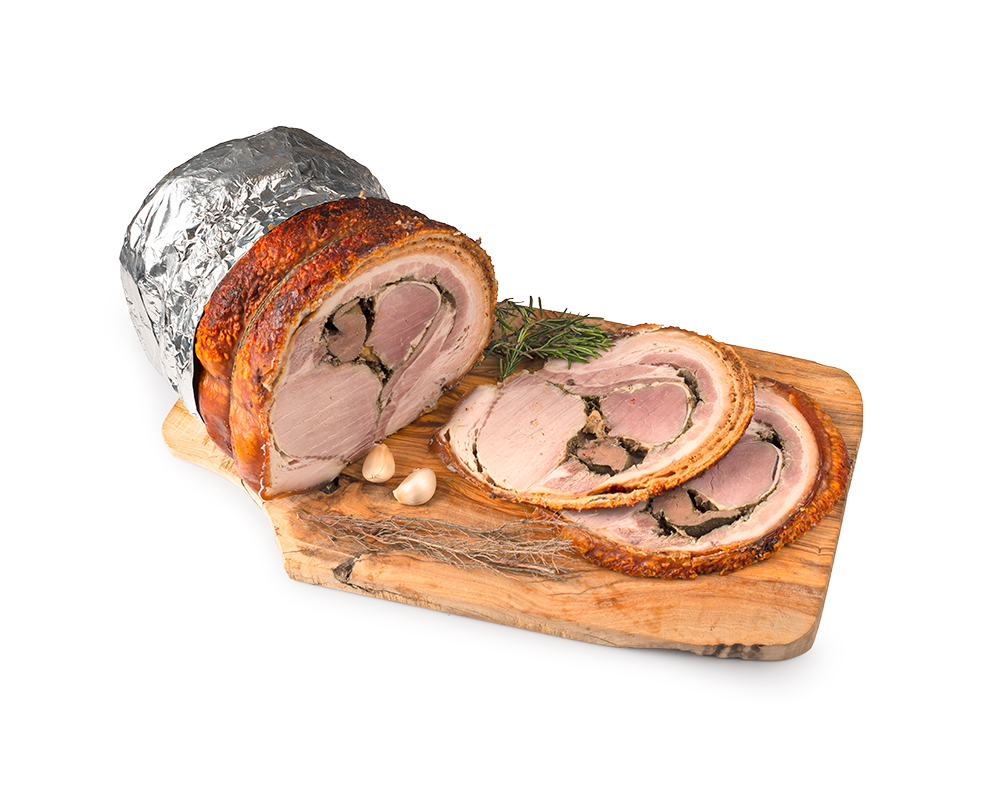
\includegraphics{../img/Tronchetto-cotto-a-legna.jpg}

}

\end{minipage}%
\newline
\begin{minipage}[t]{0.60\linewidth}
\subcaption{\label{tbl-panel-mmons-2}Finocchione }

\tabularnewline

\fontsize{9.5}{11.5}\selectfont
\begin{tabular}{>{\raggedright\arraybackslash}p{3.25cm}>{\raggedright\arraybackslash}p{2.25cm}l}
\toprule
\textbf{Prodotto} & \textbf{Quantità} & \textbf{CHF/Kg}\\
\midrule
\textbf{\em{Finocchiona}} & \textbf{10-12 kg} & \textbf{}\\
\cmidrule{1-3}
 & 1/2 o 1 & 42\\

\multirow[t]{-2}{3.25cm}{\raggedright\arraybackslash \em{Finocchiona IGP}} & >1 & 38.64\\
\bottomrule
\multicolumn{3}{l}{\rule{0pt}{1em}\textit{Note: }}\\
\multicolumn{3}{l}{\rule{0pt}{1em}Quantità indica il peso di un pezzo}\\
\multicolumn{3}{l}{\rule{0pt}{1em}}\\
\end{tabular}

\end{minipage}%
%
\begin{minipage}[t]{0.40\linewidth}

\raisebox{-\height}{

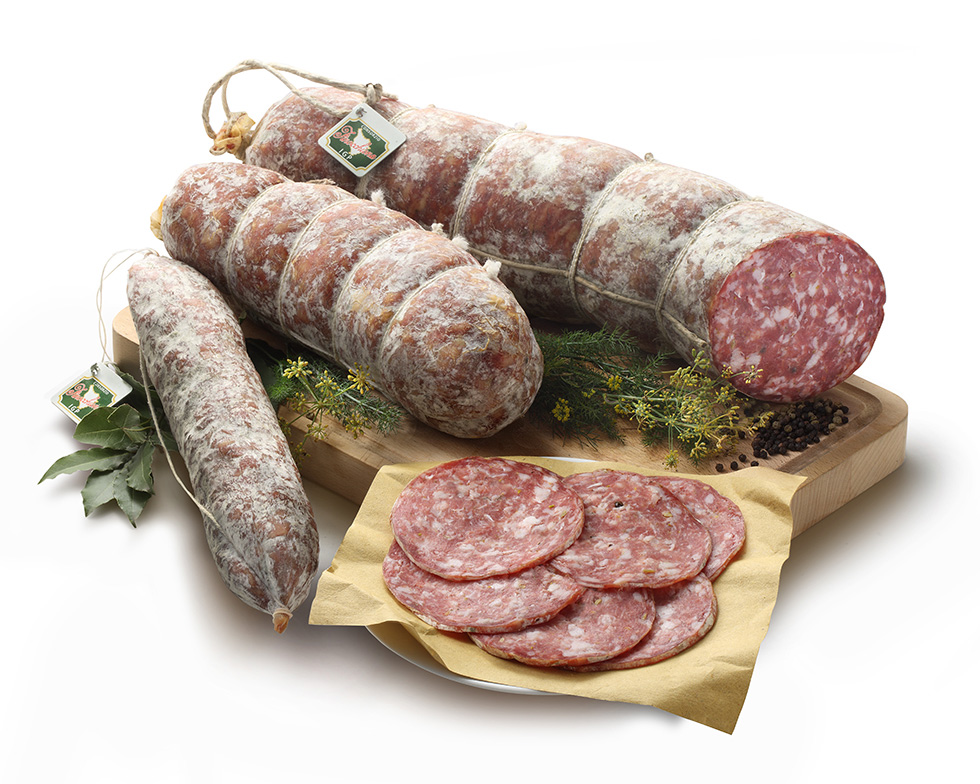
\includegraphics{../img/Finocchiona-IGP.jpg}

}

\end{minipage}%

\end{table}



\end{document}
